% This document provides the style to be used for a MSc Thesis at the
% Parallel and Distributed Systems group
\documentclass[11pt,twoside,a4paper,openright]{report}

% math packages
\usepackage{amsmath}
\usepackage{amssymb}

% textblocks for title page
\usepackage[absolute]{textpos}

% use babel for proper hyphenation
\usepackage[british]{babel}

% Graphics: different for pdflatex or dvi output, choose one
%%\usepackage[dvips]{graphicx}
\usepackage[pdftex]{graphicx}
\usepackage{graphicx}

\usepackage{epstopdf}
\usepackage{rotating}
\usepackage{subfigure}

% FONT
\usepackage[scaled=.92]{helvet}
%\usepackage{times}

% for url's use "\url{http://www.google.com/}"
\usepackage{url}
\usepackage[plainpages=false]{hyperref} 

% Information that will be filled in at various points in the report
\newcommand{\reportTitle}{A Transiently powered autonomous robot}
\newcommand{\reportAuthor}{Koen Schaper}
\newcommand{\reportEmail}{k.p.schaper@student.tudelft.nl}
\newcommand{\reportUrlEmail}{\href{mailto:\reportEmail}{\reportEmail}}
\newcommand{\reportMSC}{Embedded Systems} %{Embedded Systems}{Computer Engineering}{Computer Science}{Electrical Engineering}
\newcommand{\reportDate}{\today} %TODO: Dit is de datum van uitgifte van final versie aan de afstudeer commissie 
\newcommand{\presentationDate}{\today} %TODO: Dit is de datum van de afstudeerpresentatie 
\newcommand{\graduationCommittee}{
TODO GRADUATION COMMITTEE & Delft University of Technology \\
TODO GRADUATION COMMITTEE & Delft University of Technology \\
} % The order of listing the names: Graduation prof, supervisor(s), others ordered by title + alphabetical 
%examples: 
%prof. dr. ir. H. J. Sips (chair) & Delft University of Technology \\ 
%ir. dr. D. H. J. Epema           & Delft University of Technology \\ 
\newcommand{\reportAbstract}{TODO ABSTRACT}
\newcommand{\reportKeywords}{TODO KEYWORDS}

% For pdflatex
\pdfinfo{
   /Author (\reportAuthor)
   /Title  (\reportTitle)
   /Keywords (\reportKeywords)
}

\begin{document}

\pagenumbering{alph}
\pagestyle{empty}


% FRONTCOVER
%%\usepackage[total={210mm,297mm},left=0pt,bottom=0pt,top=0cm,right=0pt,headsep=0pt,head=0pt,showframe]{geometry}

%%\input{preambleL31958}
%%\begin{titlepage}
\begin {textblock*}{210mm}(0mm,0mm)
\noindent

\includegraphics[height=3.2cm]{pics/block}
\sffamily
\vspace{.8cm}
\begin{center}
\Large
Delft University of Technology\\
Master's Thesis in \reportMSC\\
\vspace{2cm}
\parbox{170mm}{\bfseries\centering\Huge\reportTitle}\\
\vspace{1cm}
\parbox{170mm}{\bfseries\centering\reportAuthor}

\end{center}
\end{textblock*}


\begin {textblock*}{210mm}[0.0,1.0](0mm,297mm)
\noindent

\hfill\parbox{15.5cm}{
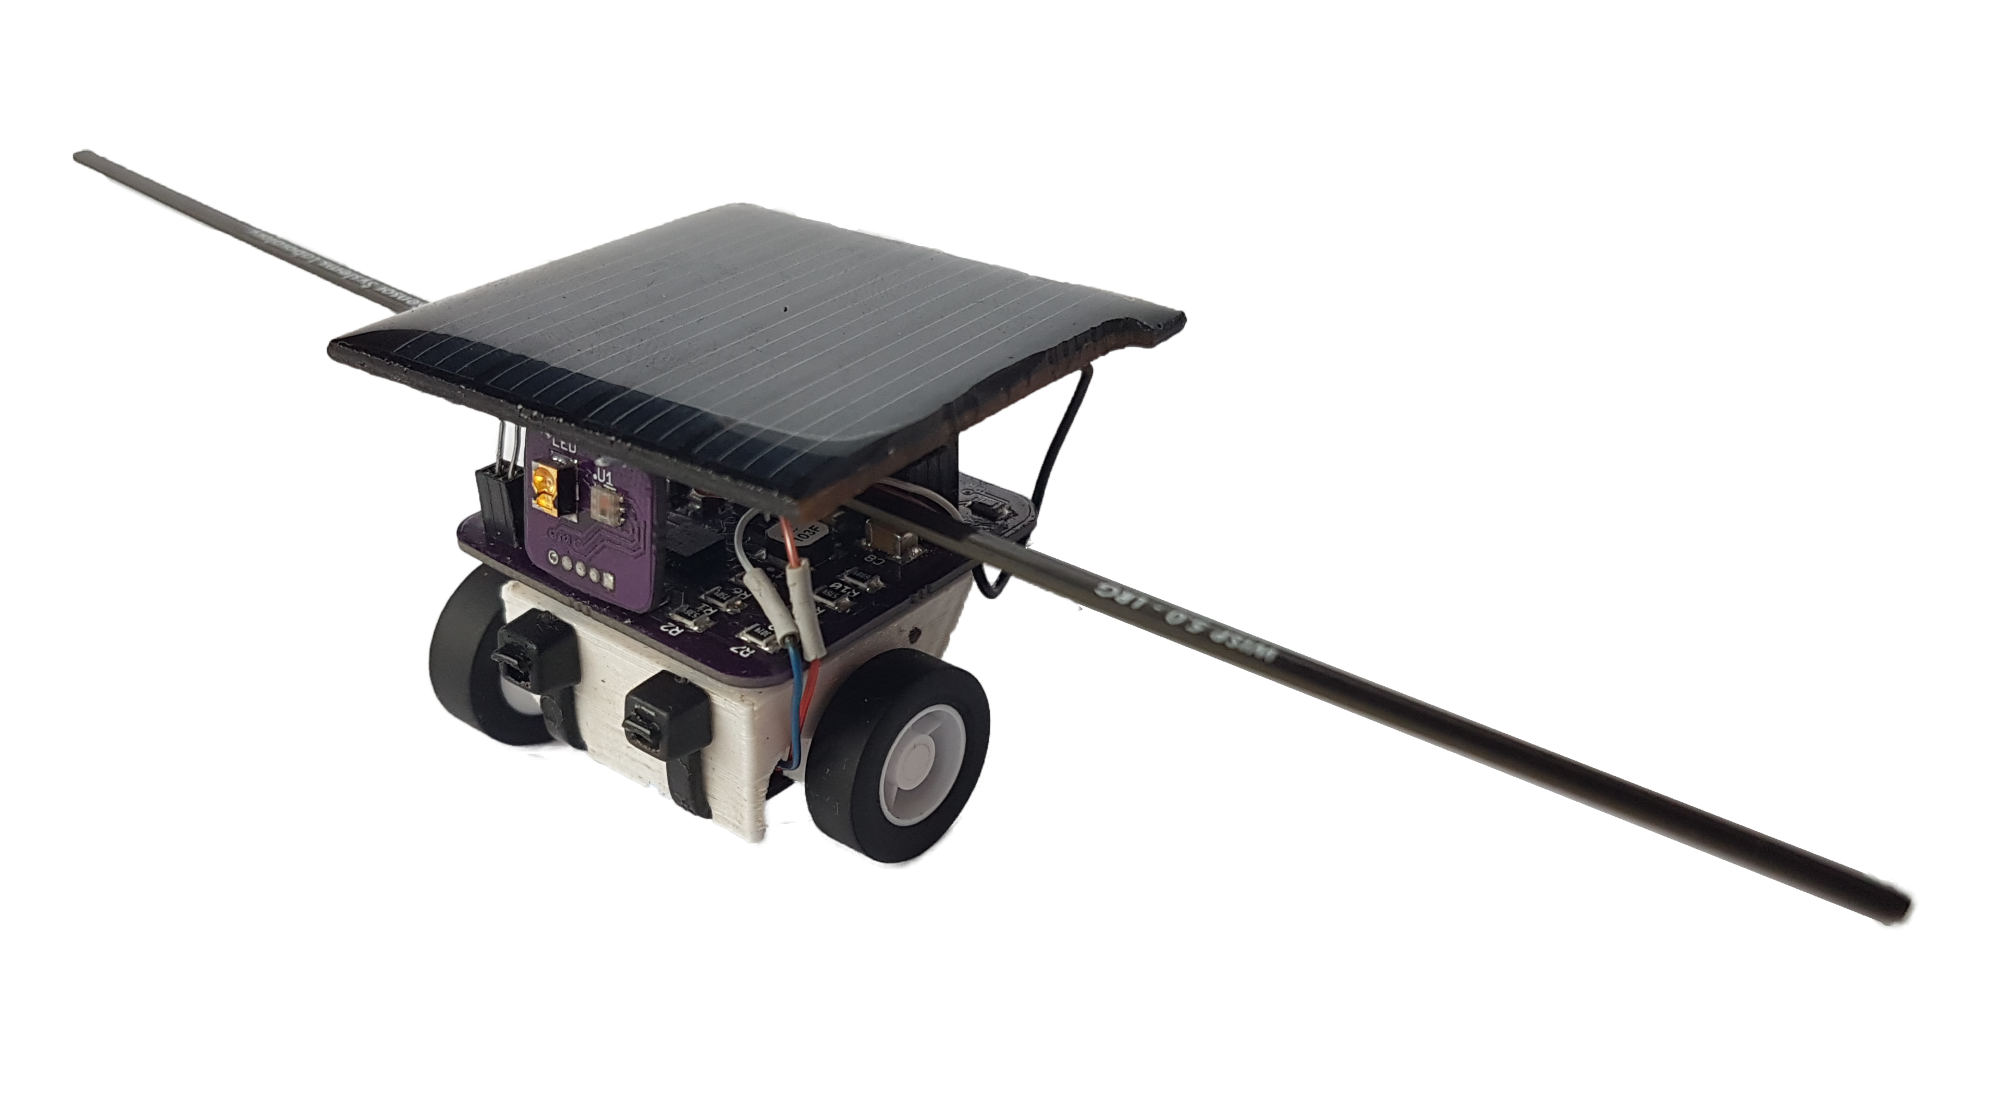
\includegraphics[width=13cm]{pics/tp_robot.png}
}
\vspace*{4cm}

\noindent
\hspace{1.89cm}
\hfill\parbox{5cm}{

\includegraphics[width=5cm]{pics/es_logo_cyan_black_rgb}}
\hspace*{2cm}\\

\vspace*{1.5cm}
\noindent

\includegraphics[width=\textwidth]{pics/TU_border_A4_L_front}
\end{textblock*}

\null\newpage


%%%%%%%%%%%%%%%%%%%%%%%%%%%%%%%%%%%%%%%%%%%%%%%%%%%%%%%%%%%%%%%%%%%%%%%%%%%%%%%
\hoffset=1.63cm
\oddsidemargin=0in
\evensidemargin=0in
\textwidth=5in

%%%%%%%%%%%%%%%%%%%%%%%%%%%%%%%%%%%%%%%%%%%%%%%%%%%%%%%%%%%%%%%%%%%%%%%%%%%%%%%
\parindent=1em

% EMPTY PAGE
\cleardoublepage

\pagestyle{plain}
\pagenumbering{roman}
\setcounter{page}{1}

% TITLE PAGE: page i (hidden)
\begin{titlepage}

  \begin{center}
  \null\vfill
    \begin{center}
    \LARGE{\reportTitle}
    \end{center}

    \vspace{3cm}

    \begin{large}
    Master's Thesis in \reportMSC
    \end{large}

    \vspace{1.5cm}

    \begin{normalsize}
    Embedded Software Section\\
    Faculty of Electrical Engineering, Mathematics and Computer Science\\
    Delft University of Technology\\
    Mekelweg 4, 2628 CD Delft, The Netherlands
    \end{normalsize}

    \vspace{2.0cm}

    \begin{normalsize}
    \reportAuthor \\
    \reportUrlEmail
    \end{normalsize}

    \vspace{1.0cm}

    % <MM> DD, YYYY
    \reportDate             %TODO: Dit is de datum van uitgifte van final versie aan de afstudeer commissie

  \vfill
  \end{center}

\end{titlepage}


% GRADUATION DATA AND ABSTRACT: pages ii and iii (hidden)
%De aankondiging bevat de spreker, titel, plaats, datum en tijd, samenstelling van de afstudeercommissie en een korte samenvatting (maximaal 25 regels).
\thispagestyle{empty}

\noindent \textbf{Author}\\
\begin{tabular}{l}
\reportAuthor{} (\reportUrlEmail)\\
\end{tabular}\\
\noindent \textbf{Title}\\
\begin{tabular}{l}
\reportTitle\\
\end{tabular}\\
\noindent \textbf{MSc presentation}\\
\begin{tabular}{l}
% <MM> DD, YYYY (like \today)
\presentationDate\\
\end{tabular}

\vspace{1.1cm}

\noindent \textbf{Graduation Committee}\\
\begin{tabular}{ll}
\graduationCommittee
\end{tabular}


\begin{abstract} %de abstract bevat alleen een korte samenvatting van de inhoud van het onderzoek
\setcounter{page}{3}
\reportAbstract{}
\end{abstract}

\clearpage

%\setcounter{page}{4}

% EMPTY PAGE: page iv
\cleardoublepage

% OPTIONAL QUOTATION: page v
%\pagestyle{empty}

\null\vfill

\begin{center}
\emph{``TODO QUOTE''} -- TODO QUOTED PERSON
\end{center}

\vspace{10cm}

\clearpage


% EMPTY PAGE: page vi
%\cleardoublepage

% PREFACE: page v
\chapter*{Preface}
\addcontentsline{toc}{chapter}{Preface}

This thesis presents the final work done towards obtaining my master’s degree in Embedded Systems from Delft University of Technology.
To the best of my knowledge no previous work has been conducted, exploring the feasibility of a transiently-powered battery-free robot. 


\vspace{1\baselineskip}

\noindent
I would like to express my sincere gratitude to my supervisor Przemys\l{}aw Pawe\l{}czak for his excellent guidance, never failing support and enthusiasm about this project. 
I also would like to thank Amjad Majid for letting me explore his idea of transiently-powered actuation, his constructive criticism and clever suggestions as this project evolved.
Moreover, I would like to thank Sinan Yildirim for his willingness to answer any of my questions, Ioannis Protonotarios for helping me with any hardware related issues, Michel Jansen for sharing his schematics.
Additionally, I would like to thank the Nuon Solar Team for lending me one of their space grade solar panels from their 2017 Nuna9 solar car.
Furthermore, I want to thank Prof. Koen Langendoen for hosting me at the Embedded Systems group, and Javier Alonso-Mora for participating as a member of my graduation committee.
Last but not least, a special thanks to my family for their unconditional support, encouragements and love that helped me stay motivated during this year.

\vspace{1\baselineskip}

\noindent
Koen Schaper

\vspace{1\baselineskip}

\noindent
Delft, The Netherlands

\noindent
\today

% EMPTY PAGE: page vi
\cleardoublepage

% TABLE OF CONTENTS: starting at page vii
\tableofcontents

\cleardoublepage

\pagenumbering{arabic}
\setcounter{page}{1}

% INTRODUCTION: page 1
\chapter{Introduction}
\label{chp:introduction}

% printer: Tethered flight control of a small quadrotor robot for stippling \cite{galea_iros_2017}

% Estabish your territory

Miniature robots with limited capabilities can work together in "swarms" to achieve more than an individual could by itself, but are still far from being applicable in real world applications~\cite{barca_sekercioglu_2013}.
The future potential of swarms is widely recognized to have applications in surveillance, search and rescue, and exploration.
Swarms have been proposed as a new form of user interface, robots can display information and interact with users on tabletops~\cite{legoc_uist_2016}, unmodified clothing~\cite{dementyev_uist_2016} and can be an educational toy for kids~\cite{sony_toio_2017}.
\hfill \break

% Establish nice
% Motivation for this work: Why do we want to remove the battery?

However, one of the fundamental issues that needs to be addressed before swarm robotics can advance is related to energy, small lithium batteries are currently powering the robots and limit their operation time to only a view hours. 
The energy density of batteries has improved less than 1 order of magnitude since 1945, in comparison the energy efficiency of computing has improved 12 orders of magnitude~\cite{patel_pvc_2017}.
The last major advancement in battery technology is 25 years old and came with the introduction of Li-ion batteries.
Additionally, any new big improvements in energy density of batteries is not likely to happen anytime soon, as new battery technologies are often overhyped and slow to emerge~\cite{zachary_spec_2016}.
\hfill \break

%TODO introduce current research

% Propose a solution: Energy harvesting
% And discuss current solutions to autonomus operation / battery replenishment

A stable energy supply is a current requirement to allow long term persistent autonomous operation of swarm robots.
Relaxing this constraint by allowing a transient supply of energy could be a potent area of research.
Wireless sensor nodes that rely on energy harvesting have already been emerging, some are highly energy constrained but fully eliminate the need for batteries.
In contrary, different replenishment methods for robot batteries are currently used, robots can be moved to a charging station leaving them nonoperational while recharging or the battery could be replaced, resulting in a high strain on maintenance.

% 4 lines left!
\newpage

\section{Problem statement}

% What why how

% Intermittently powered robots, that purely rely on harvested power are currently non existent.

Replacing a robots battery with an energy harvesting system could make it more self sufficient and energy-autonomous. 
This however introduces a new phenomenon to take into account; the intermittent availability of energy produces frequent power interrupts.
The possibility of sudden power loss is currently not considered when developing software that controls a robots behavior, and for this reason can not be used without adaption.
\hfill \break

Secondly, sensors and control techniques used may not be found applicable due to energy budget constrains or their inability to be interrupted by a loss of power. 
Different locomotion types are used and may not all be reliable and/or accurate under the frequent power interruption.
This research will explore the feasibility of a miniature battery-less robot, allowing persistent operation while being supplied with a small and intermittent source of energy.
Therefore the main question this work will try to answer is:

\begin{center}
	\textit{How to enable a transiently powered robot to operate autonomously?}
\end{center}

\section{Contributions}
Current swarm robots assume that a task can only be completed if sufficient energy is left in the batteries, which also limits their operation time. 
While surprisingly this is the first study of transiently powered robots, unaware of any platforms being implemented and are operating under the constant threat of power loss. 

\begin{enumerate}

%\item A simple model is developed showing the relation between the energy stored, weight of the robot, frequency of power cycles and distance covered with a single charge.

\item Design of a battery-less robot that purely operates from harvested energy, with basic capabilities allowing autonomous operation.

\item Implementation of a control algorithm, that allows the robot to finish a movement across power cycles.

%\item Evaluation of the battery-less robot compared to a battery powered robot in terms of, weight, speed and accuracy of movement.


\end{enumerate}


\section{Thesis Outline}
%What will be discussed in the coming chapters


\vspace{1\baselineskip}

\noindent
TODO ORGANISATIONAL DESCRIPTION OF THESIS



\chapter{Related Work}
\label{chp:related_work}

This chapter will provide background information about current state of the art transiently powered systems. The advantages and disadvantages of different electrical storage types are compared. A short summary of current miniature robotics platforms is given and commonly used locomotion types. Finally different methods that try to ensure continuous operation will be discussed.

\section{Transiently-powered systems}
\label{sec:tp_systems}

% - Roughly everything that is powered fron a Energy harvester

Example of energy harvesting: Prolonged energy harvesting for ingestible devices~\cite{plonski_tranro_2016}
Drug delivery
\\
Converting a Plant to a Battery and Wireless Sensor with Scatter Radio and Ultra-Low Cost

%Other sources available for exploration are often limited by the application. Secondly, most sources can be scarce or completely absent during prolonged time intervals of the day as well \cite{RN15}. 

Fully programmable RFID platforms have been developed to exploring the combination of sensing, computation and communication, while allowing battery-less operation by harvesting RF energy~\cite{sample_transim_2008}.
The amount of energy collected from RF signals is very small and decreases with the distance of the device to the transmitter.
The harvested energy is typically stored in a capacitor, where larger capacitors can buffer more energy and smaller capacitors have the advantage of shorter charge times~\cite{gummerson_mobisys_2010}.
For longer, complex operations the energy budged needs to be evaluated carefully.
To store the energy an appropriate size storage capacitor needs to be selected~\cite{naderiparizi_rfid_2015}.

% - Short intro into persistent framwork: checkpointing etc
% mementos
% chain
% ratchet

\section{Energy Supply}
\label{sec:energy_supply}

% Explain battery vs supercapacitor

Comparing li-ion batteries with super-capacitors there are some big differences.
Supercapacitors do not need any special charging scheme and circuity for charging, except for overcharging protection.
Secondly, super-capacitors do not require any particular current profile, the energy can be stored at any rate and when the energy is required it can be extracted at any power level.
Operating a li-ion battery outside of it's recommended operating conditions can severely reduce a batteries lifetime and result in overheating or even explosion of the battery.
Batteries will seldom withstand more than one thousand complete charge/discharge cycles.
Super-capacitors used under extreme condition's, are not likely to explode but instead rupture.
While the biggest disadvantages of super-capacitors is their low energy density and high price, their lifetime is typically hundred thousands of charge/discharge cycles.

Li-Ion Battery-Supercapacitor Hybrid Storage System for a Long Lifetime, Photovoltaic-Based Wireless Sensor Network	\cite{ongaro_pwre_2012}
Reincarnation in the Ambiance: Devices and Networks with Energy Harvesting \cite{prasad_comst_2014}



\section{Small robotic platforms}
\label{sec:robotic_platforms}

%TODO tell that these robots are used for studing swarm behavior (inspired by nature)
% require communication to apply different algorithms
% need to be low cost and size are key factors for allowing scalability
% 
%Main characteristics : https://link.springer.com/article/10.1007/s11721-012-0075-2
%robots are autonomous;
%robots are situated in the environment and can act to modify it;
%robots’ sensing and communication capabilities are local;
%robots do not have access to centralized control and/or to global knowledge;
%robots cooperate to tackle a given task.

Low cost robotic platforms have been developed to tackle a variety of challenges anonymously.
Miniature robots can be used for inspection in difficult to reach places, operating like mobile sensing units.
Hardware modularity is a way to make the robot adapt its resources to different environments and sensing operations.
By separating out power, computation, motor control and sensing a verity of capabilities can be tested~\cite{sabelhaus_icra_2013, pickem_icra_2015, kim_iros_2016}.
Microrobots typically use infrared-based neighbor to neighbor distance sensing and communication~\cite{rubenstein_icra_2012, pickem_icra_2015, kim_iros_2016}.
While controlling a swarm or collective is mainly accomplished by means of active low power transceivers~\cite{sabelhaus_icra_2013, pickem_icra_2015, kim_iros_2016}. 

%TODO reference table

\section{Locomotion}
\label{sec:locomotion}
%TODO tell somthing about their accuracy!

Choosing the right locomotion resource can depend on different factors, moving in the most energy efficient way on a particular surface is often the determining factor.
On a flat surface, robots commonly use a two-wheeled differential drive design to not only move but allow for steering as well~\cite{sabelhaus_icra_2013, pickem_icra_2015}.
The GRITSBot does not use conventional DC motors, requiring encoders to estimate their speed. 
Instead by using stepper motors the speed can be set by changing the delay between steps. 
Estimating it's position therefore is reduced to simply counting steps~\cite{pickem_icra_2015}.  
Overall cost can be a decisive factor, therefore the Kilobot uses two vibrating motors for locomotion combined with three thin legs.
When the motors are activated the centripetal forces will generate a forward movement, which can be explained using the slip-stick principle~\cite{rubenstein_icra_2012}.
Other locomotion types are biologically inspired, the HARM-VP is small scale piezoelectric driven quadrupled robot~\cite{baisch_iros_2013}.
Each leg as two degrees of freedom, it can move up and down, as well as forward and backward.

\section{Continuous operation}
\label{sec:continous_operation}
%Battery replenishment

%TODO include battery tosti iron anecdote
Typically the operation time is extended by regularly checking the remaining energy in the battery and move to a recharging station before the robot runs out of energy~\cite{pickem_icra_2015, rubenstein_icra_2012}.
As an alternative to quickly recharging, the battery can also be swapped automatically when the robot moves into the docking station~\cite{kemal_mech_2015}.
Another work shows a robot which is able to swap it's primary battery using a six degree-of-freedom manipulator, used to grab the dead battery and plug it into a wireless recharging charging station \cite{zhang_conel_2013}.
Using direct wireless power to replace or supplement to a batteries energy is shown in~\cite{karpelson_icra_2014}, however the robot can only operate or recharge while remaining in close proximity to a transmitter. 
In these cases the robots are highly reliant on an infrastructure to allow for continuous autonomous operation.
This can be a severe constraint if the robot moves out of reach or needs to operate in a area where this infrastructure is not present. Persistent operation can also be achieved by harvesting renewable energy, particularly solar energy to complement to the robots internal energy source. To remove weight from the robot, in \cite{bruhwiler_iros_2015} the solar energy is used directly without any type of energy buffer. A drawback of this method is that the incoming solar energy should already greater or equal to the energy required for operation. This approach has been tested for basic locomotion and did not combine any form of sensing and control.

% - Provide overview table robots smaller than 15*15cm

% For each of these cases you need to provide numbers: 
% level of autonomy (does the robot does all by itself or relies on external processing)
% does autonomy fall under 
% charging time

% Add missing "new" robots

\begin{table*}[t]
	\centering
	\tiny
	\begin{threeparttable}
		\caption{An comparison of small robotic platforms}
		\label{tab:comparison_robot_platforms}
 		\begin{tabularx}{\textwidth}{l l X X X l l l} 
			\hline
 			Robot & Cost & Scalability & Sensors & Locomotion & Size [cm] & Weight [g] & Battery life \\ 
 			\hline
 			IPR & TBD & charge, program & gyro, distance, ambient light & wheel, 25cm/s & 4.0 & 21 & 1s\\
 			HAMR-VP\textsuperscript{1} \cite{bruhwiler_iros_2015} & NS & none & gyroscope, optical mouse & legged, 1cm/s & 4.4 & 2.3 & 3m \\
 			Roverables \cite{dementyev_uist_2016} & NS & charge & wheel, distance, optical encoders & wheel, ?? & 4.0 & ?? & 45m \\ 
 			Zooids \cite{legoc_uist_2016} & \$50 & ?? & position, touch & wheel, 50cm/s & 2.6 & 12 & 1-2h \\ 
 			mROBerTO \cite{kim_iros_2016} & \$60\textsuperscript{1} & program & light, range, gyro, camera, accel., compass, distance, bearing & motor shaft, 15cm/s & 1.5 & ?? & 1.5h\\
 			GRITSBot \cite{pickem_icra_2015} & \$50\textsuperscript{2} & charge, program, calibrate & distance, bearing, 3d accel., 3d gyro & wheel, 25cm/s & 3 & ?? & 1-5h \\
 			Kilobot \cite{rubenstein_icra_2012} & \$50\textsuperscript{2} & charge, program & distance, ambient light & vibration, 1cm/s & 3.3 & ?? & 3-24h\\
 			TinyTerp \cite{sabelhaus_icra_2013} & \$50 & none & 3d gyro, 3d accel. & wheel, 50cm/s & 1.8 & ?? & 1h\\
			\hline
		\end{tabularx}
		\begin{tablenotes}
			\item [1] Modified to include on-board power, sensing and control.
			\item [2] Cost of parts
		\end{tablenotes}
	\end{threeparttable}
\end{table*}

% CHAPTERS ... For instance: History/Prior Work, Design/Implementation, Experiments
\chapter{CHAPTER TITLE}
\label{chp:CHAPTERTITLE}
INTRODUCTION TEXT TO THIS CHAPTER IN WHICH ALL SECTIONS ARE DESCRIBED ROUGHLY (1 SENTENCE EACH).

This chapter describes the ... In Section~\ref{sec:SECTIONTITLE}, examples are given of how to use tables and figures in MSc theses.

\section{SECTION TITLE}
\label{sec:SECTIONTITLE}

Every caption of a table (or figure) should start with a capital letter, and should end with a period. References to tables are given with a capital letter for table, as in ``(see Table~\ref{tab:EXAMPLETABLE})'' or ``in Table~\ref{tab:EXAMPLETABLE}, ...''.

\begin{table}[htb]
\centering
\begin{tabular}{|l|c|r|}
\hline % horizontal line
left aligned & centred & right aligned \\
\hline \hline
12           & 34      & 56            \\
\hline
\end{tabular}
\caption{Complete sentence describing the tabular data.}
\label{tab:EXAMPLETABLE}
\end{table}

References to figures are given with a capital letter for figure, as in ``(see Figure~\ref{fig:EXAMPLEFIGURE})'' or ``in Figure~\ref{fig:EXAMPLEFIGURE}, ...''.

\cite{b}
\cite{a}

\begin{figure}[htb]
% most GNUplot figures need to be rotated, width should be the same throughout the complete document, and no extension is needed

\includegraphics[angle=180,width=\textwidth]{pics/TUD_logo_zw}
\caption{Complete sentence describing the figure thoroughly.}
\label{fig:EXAMPLEFIGURE}
\end{figure}



% CONCLUSIONS AND FUTURE WORK
\chapter{Conclusions and Future Work}
\label{chp:conclusionsandfuturework}

\section{Conclusions}
TODO CONCLUSIONS

\section{Future Work}
TODO FUTURE WORK



% BIBLIOGRAPHY
%#define SORTED 1
\bibliographystyle{../bib/latex8}
\bibliography{../bib/mycollection}

%\appendix

%\chapter{TODO APPENDIX NAME}
\label{app:}
Appendix body



\end{document}

